%!TEX root = skripsi.tex
%-----------------------------------------------------------------------------%
\chapter{\babLima}
%-----------------------------------------------------------------------------%

Sistem pengenalan suara otomatis pada penelitian ini adalah sistem pengenalan per ayat. Bab \ref{eksperimen} menjelaskan bagaimana eksperimen dilakukan terhadap satu ayat. Setiap ayat mendapat perlakuan sama dalam eksperimen. Pengujian suatu ayat akan menghasilkan sebuah \f{confusion matrix}, lalu dari \f{confusion matrix} diperoleh metrik evaluasi berupa nilai akurasi, presisi, \f{recall}, dan \f{f-measure}. Banyaknya ayat yang diproses dalam eksperimen yang sudah dilakukan adalah 564 ayat, sehingga akan dihasilkan pula 564 metrik evaluasi tersebut.

Untuk menampilkan keseluruhan data hasil eksperimen secara ringkas, data tersebut disajikan dalam bentuk histogram. Sumbu X pada histogram menyatakan interval persentase, sedangkan sumbu Y pada histogram menyatakan banyaknya hasil eksperimen yang berada pada interval tersebut. Contoh interval dalam histogram yang disajikan adalah (90\%,95\%]. Interval tersebut merepresentasikan rentang \f{lebih dari} 90\% dan \f{kurang dari atau sama dengan} 95\%. Semakin tinggi \f{bar} histogram akurasi pada interval (90\%,95\%], artinya semakin banyak ayat yang berhasil diklasifikasikan oleh sistem dengan $90\%<\text{akurasi}\leq95\%$. Jadi jika pada suatu metode, \f{bar} histogram tinggi berkumpul pada interval tinggi, menunjukkan bahwa metode tersebut baik. Sebaliknya, jika \f{bar} histogram tinggi berkumpul pada interval rendah, menunjukkan bahwa metode tersebut kurang baik.

%-----------------------------------------------------------------------------%
\section{Hasil dengan Fitur MFCC}
%-----------------------------------------------------------------------------%

  %-----------------------------------------------------------------------------%
  \subsection{Hasil dengan Fitur MFCC dan Metode Klasifikasi SVM}
  %-----------------------------------------------------------------------------%
  Eksperimen menggunakan fitur MFCC dan menggunakan metode klasifikasi SVM, memberikan hasil yang dirangkum pada Tabel \ref{table:mfccsvm} berikut.

  \begin{table}
    \centering
    \caption{Rangkuman Hasil Eksperimen dengan Fitur MFCC dan Metode Klasifikasi SVM}
    \begin{tabular}{|c|c|c|c|c|}
      \hline
       & Akurasi & Presisi & \f{\f{Recall}} & \f{\f{F-Measure}} \\ \hline
      Minimal         & 41.3\% & 42.2\% & 42.5\% & 44.4\% \\ \hline
      Maksimal        & 87.5\% & 96.2\% & 82.5\% & 86.8\% \\ \hline
      Rata-rata       & 63.1\% & 63.7\% & 63.0\% & 63.1\% \\ \hline
      Standar Deviasi & 7.24\% & 8.09\% & 7.75\% & 6.86\%  \\ \hline
    \end{tabular}
    \label{table:mfccsvm}
  \end{table}

  Tabel \ref{table:datahistogram00} menunjukkan frekuensi kemunculan persentase tertentu yang dikelompokkan ke dalam interval 5\%.

  \begin{table}
    \centering
    \caption{Frekuensi Kemunculan Interval Persentase pada Eksperimen dengan Fitur MFCC dan Metode Klasifikasi SVM}
    \begin{tabular}{|c|c|c|c|c|}
      \hline
\multicolumn{1}{|c|}{Persentase} & \multicolumn{1}{c|}{\begin{tabular}[c]{@{}c@{}}Frekuensi\\ Nilai Akurasi\end{tabular}} & \multicolumn{1}{c|}{\begin{tabular}[c]{@{}c@{}}Frekuensi\\ Nilai Presisi\end{tabular}} & \multicolumn{1}{c|}{\begin{tabular}[c]{@{}c@{}}Frekuensi\\ Nilai \f{Recall}\end{tabular}} & \multicolumn{1}{c|}{\begin{tabular}[c]{@{}c@{}}Frekuensi\\ Nilai \f{F-Measure}\end{tabular}} \\ \hline
(40\%,45\%{]}  & 6   & 5   & 8   & 2   \\ \hline
(45\%,50\%{]}  & 16  & 17  & 33  & 15  \\ \hline
(50\%,55\%{]}  & 55  & 51  & 67  & 51  \\ \hline
(55\%,60\%{]}  & 120 & 112 & 120 & 114 \\ \hline
(60\%,65\%{]}  & 167 & 148 & 141 & 171 \\ \hline
(65\%,70\%{]}  & 122 & 130 & 121 & 126 \\ \hline
(70\%,75\%{]}  & 52  & 51  & 42  & 58  \\ \hline
(75\%,80\%{]}  & 21  & 30  & 29  & 22  \\ \hline
(80\%,85\%{]}  & 4   & 15  & 3   & 4   \\ \hline
(85\%,90\%{]}  & 1   & 2   & 0   & 1   \\ \hline
(90\%,95\%{]}  & 0   & 2   & 0   & 0   \\ \hline
(95\%,100\%{]} & 0   & 1   & 0   & 0   \\ \hline
    \end{tabular}
    \label{table:datahistogram00}
  \end{table}

  Gambar \ref{fig:histogram00} merepresentasikan Tabel \ref{table:datahistogram00} dalam bentuk histogram.
  \begin{figure}
    \centering
    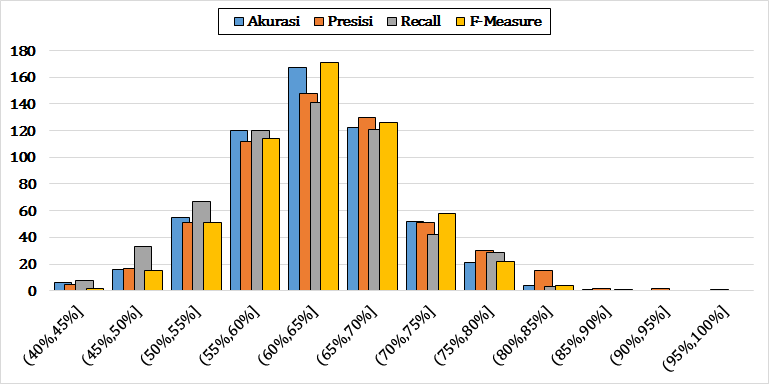
\includegraphics[width=\linewidth]{pics/histogram00}
    \caption{Histogram Metrik Evaluasi dengan Fitur MFCC dan Metode Klasifikasi SVM}
    \label{fig:histogram00}
  \end{figure}

  Dari Gambar \ref{fig:histogram00} dapat diamati bahwa mayoritas ayat dalam eksperimen terklasifikasi dengan rentang akurasi (60\%,65\%].




  %-----------------------------------------------------------------------------%
  \subsection{Hasil dengan Fitur MFCC dan Metode Klasifikasi GMM}
  %-----------------------------------------------------------------------------%
  Eksperimen menggunakan fitur MFCC dan menggunakan metode klasifikasi GMM, memberikan hasil yang dirangkum pada Tabel \ref{table:mfccgmm} berikut.

  \begin{table}
    \centering
    \caption{Rangkuman Hasil Eksperimen dengan Fitur MFCC dan Metode Klasifikasi GMM}
    \begin{tabular}{|c|c|c|c|c|}
      \hline
       & Akurasi & Presisi & \f{\f{Recall}} & \f{\f{F-Measure}} \\ \hline
      Minimal         & 43.8\% & 43.9\% & 42.5\% & 44.4\% \\ \hline
      Maksimal        & 85.0\% & 93.3\% & 90.0\% & 85.0\% \\ \hline
      Rata-rata       & 65.8\% & 66.3\% & 65.1\% & 65.4\% \\ \hline
      Standar Deviasi & 6.50\% & 7.19\% & 8.56\% & 6.72\%  \\ \hline
    \end{tabular}
    \label{table:mfccgmm}
  \end{table}

  Tabel \ref{table:datahistogram01} menunjukkan frekuensi kemunculan persentase tertentu yang dikelompokkan ke dalam interval 5\%.

  \begin{table}
    \centering
    \caption{Frekuensi Kemunculan Interval Persentase pada Eksperimen dengan Fitur MFCC dan Metode Klasifikasi GMM}
    \begin{tabular}{|c|c|c|c|c|}
      \hline
\multicolumn{1}{|c|}{Persentase} & \multicolumn{1}{c|}{\begin{tabular}[c]{@{}c@{}}Frekuensi\\ Nilai Akurasi\end{tabular}} & \multicolumn{1}{c|}{\begin{tabular}[c]{@{}c@{}}Frekuensi\\ Nilai Presisi\end{tabular}} & \multicolumn{1}{c|}{\begin{tabular}[c]{@{}c@{}}Frekuensi\\ Nilai \f{Recall}\end{tabular}} & \multicolumn{1}{c|}{\begin{tabular}[c]{@{}c@{}}Frekuensi\\ Nilai \f{F-Measure}\end{tabular}} \\ \hline
(40\%,45\%{]}  & 2   & 1   & 6   & 1   \\ \hline
(45\%,50\%{]}  & 3   & 4   & 16  & 7   \\ \hline
(50\%,55\%{]}  & 27  & 21  & 54  & 22  \\ \hline
(55\%,60\%{]}  & 89  & 92  & 115 & 97  \\ \hline
(60\%,65\%{]}  & 144 & 116 & 137 & 146 \\ \hline
(65\%,70\%{]}  & 169 & 181 & 111 & 151 \\ \hline
(70\%,75\%{]}  & 94  & 91  & 63  & 95  \\ \hline
(75\%,80\%{]}  & 31  & 38  & 37  & 40  \\ \hline
(80\%,85\%{]}  & 5   & 15  & 19  & 5   \\ \hline
(85\%,90\%{]}  & 0   & 4   & 6   & 0   \\ \hline
(90\%,95\%{]}  & 0   & 1   & 0   & 0   \\ \hline
(95\%,100\%{]} & 0   & 0   & 0   & 0   \\ \hline
    \end{tabular}
    \label{table:datahistogram01}
  \end{table}
  
  Gambar \ref{fig:histogram01} merepresentasikan Tabel \ref{table:datahistogram01} dalam bentuk histogram.
  \begin{figure}
    \centering
    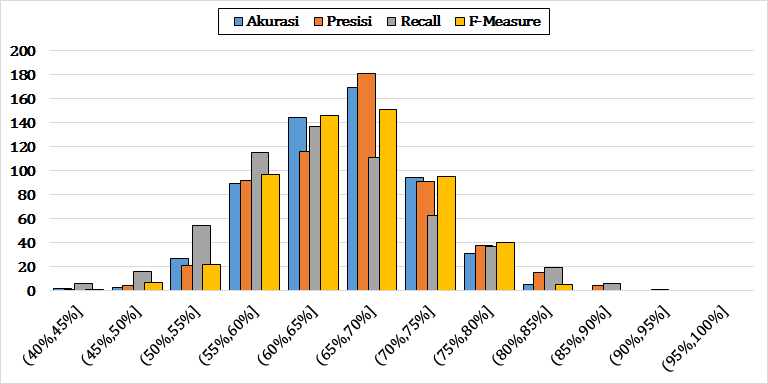
\includegraphics[width=\linewidth]{pics/histogram01}
    \caption{Histogram Metrik Evaluasi dengan Fitur MFCC dan Metode Klasifikasi GMM}
    \label{fig:histogram01}
  \end{figure}

  Dari Gambar \ref{fig:histogram01} dapat diamati bahwa mayoritas ayat dalam eksperimen terklasifikasi dengan rentang akurasi (65\%,70\%]. Hasil tersebut sedikit lebih tinggi jika dibandingkan dengan hasil pada eksperimen yang menggunakan fitur MFCC dan metode klasifikasi SVM. Hal tersebut mengindikasikan bahwa metode klasifikasi GMM lebih tepat untuk digunakan dalam sistem evaluasi pembacaan \quran~dalam penelitian ini.

  %-----------------------------------------------------------------------------%
  \subsection{Hasil dengan Fitur MFCC dan Metode Klasifikasi Gabungan}
  %-----------------------------------------------------------------------------%
  Eksperimen menggunakan fitur MFCC dengan metode klasifikasi gabungan antara SVM dan GMM, memberikan hasil yang dirangkum pada Tabel \ref{table:mfccgabungan} berikut.

  \begin{table}
    \centering
    \caption{Rangkuman Hasil Eksperimen dengan Fitur MFCC dan Metode Klasifikasi Gabungan}
    \begin{tabular}{|c|c|c|c|c|}
      \hline
       & Akurasi & Presisi & \f{\f{Recall}} & \f{\f{F-Measure}} \\ \hline
      Minimal         & 41.3\% & 42.2\% & 37.5\% & 43.9\% \\ \hline
      Maksimal        & 85.0\% & 90.0\% & 85.0\% & 84.2\% \\ \hline
      Rata-rata       & 63.5\% & 64.1\% & 63.1\% & 63.4\% \\ \hline
      Standar Deviasi & 7.64\% & 8.71\% & 8.00\% & 7.26\%  \\ \hline
    \end{tabular}
    \label{table:mfccgabungan}
  \end{table}

  Tabel \ref{table:datahistogram02} menunjukkan frekuensi kemunculan persentase tertentu yang dikelompokkan ke dalam interval 5\%.

  \begin{table}
    \centering
    \caption{Frekuensi Kemunculan Interval Persentase pada Eksperimen dengan Fitur MFCC dan Metode Klasifikasi Gabungan}
    \begin{tabular}{|c|c|c|c|c|}
      \hline
\multicolumn{1}{|c|}{Persentase} & \multicolumn{1}{c|}{\begin{tabular}[c]{@{}c@{}}Frekuensi\\ Nilai Akurasi\end{tabular}} & \multicolumn{1}{c|}{\begin{tabular}[c]{@{}c@{}}Frekuensi\\ Nilai Presisi\end{tabular}} & \multicolumn{1}{c|}{\begin{tabular}[c]{@{}c@{}}Frekuensi\\ Nilai \f{Recall}\end{tabular}} & \multicolumn{1}{c|}{\begin{tabular}[c]{@{}c@{}}Frekuensi\\ Nilai \f{F-Measure}\end{tabular}} \\ \hline
(40\%,45\%{]}  & 5   & 3   & 10  & 4   \\ \hline
(45\%,50\%{]}  & 19  & 21  & 25  & 14  \\ \hline
(50\%,55\%{]}  & 64  & 60  & 84  & 57  \\ \hline
(55\%,60\%{]}  & 115 & 116 & 109 & 116 \\ \hline
(60\%,65\%{]}  & 145 & 128 & 132 & 143 \\ \hline
(65\%,70\%{]}  & 104 & 100 & 119 & 119 \\ \hline
(70\%,75\%{]}  & 83  & 73  & 55  & 85  \\ \hline
(75\%,80\%{]}  & 24  & 39  & 26  & 21  \\ \hline
(80\%,85\%{]}  & 5   & 16  & 4   & 5   \\ \hline
(85\%,90\%{]}  & 0   & 8   & 0   & 0   \\ \hline
(90\%,95\%{]}  & 0   & 0   & 0   & 0   \\ \hline
(95\%,100\%{]} & 0   & 0   & 0   & 0   \\ \hline
    \end{tabular}
    \label{table:datahistogram02}
  \end{table}
  
  Gambar \ref{fig:histogram02} merepresentasikan Tabel \ref{table:datahistogram02} dalam bentuk histogram.
  \begin{figure}
    \centering
    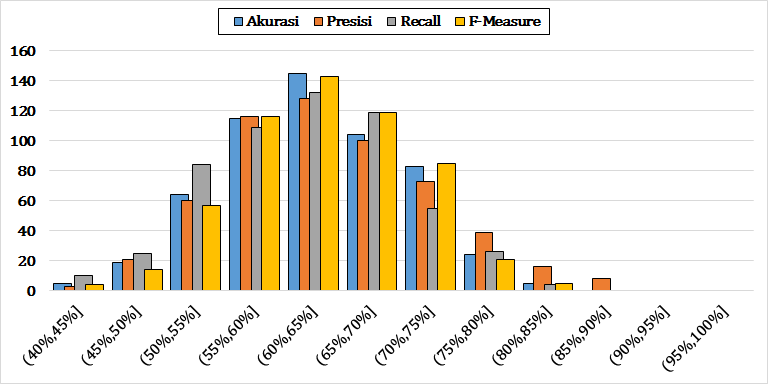
\includegraphics[width=\linewidth]{pics/histogram02}
    \caption{Histogram Metrik Evaluasi dengan Fitur MFCC dan Metode Klasifikasi Gabungan}
    \label{fig:histogram02}
  \end{figure}

  Dari Gambar \ref{fig:histogram02} dapat diamati bahwa mayoritas ayat dalam eksperimen terklasifikasi dengan rentang akurasi (60\%,65\%]. Hasil tersebut sedikit lebih rendah jika dibandingkan dengan hasil pada eksperimen yang menggunakan fitur MFCC dan metode klasifikasi GMM. Hal tersebut mengindikasikan bahwa gabungan dua metode klasifikasi, yaitu SVM dengan GMM, tidak lebih tepat untuk digunakan dalam sistem evaluasi pembacaan \quran~dalam eksperimen ini jika dibandingkan dengan metode klasifikasi GMM.





%-----------------------------------------------------------------------------%
\section{Hasil dengan Fitur SDCC}
%-----------------------------------------------------------------------------%

  %-----------------------------------------------------------------------------%
  \subsection{Hasil dengan Fitur SDCC dan Metode Klasifikasi SVM}
  %-----------------------------------------------------------------------------%
  Eksperimen menggunakan fitur SDCC dan menggunakan metode klasifikasi SVM, memberikan hasil yang dirangkum pada Tabel \ref{table:sdccsvm} berikut.

  \begin{table}
    \centering
    \caption{Rangkuman Hasil Eksperimen dengan Fitur SDCC dan Metode Klasifikasi SVM}
    \begin{tabular}{|c|c|c|c|c|}
      \hline
       & Akurasi & Presisi & \f{\f{Recall}} & \f{\f{F-Measure}} \\ \hline
      Minimal         & 51.3\% & 51.2\%  & 30.0\%  & 43.6\% \\ \hline
      Maksimal        & 96.3\% & 100.0\% & 100.0\% & 96.4\% \\ \hline
      Rata-rata       & 77.3\% & 76.6\%  & 79.5\%  & 77.8\% \\ \hline
      Standar Deviasi & 7.47\% & 8.18\% & 8.74\% & 7.41\%  \\ \hline
    \end{tabular}
    \label{table:sdccsvm}
  \end{table}

  Tabel \ref{table:datahistogram10} menunjukkan frekuensi kemunculan persentase tertentu yang dikelompokkan ke dalam interval 5\%.

  \begin{table}
    \centering
    \caption{Frekuensi Kemunculan Interval Persentase pada Eksperimen dengan Fitur SDCC dan Metode Klasifikasi SVM}
    \begin{tabular}{|c|c|c|c|c|}
      \hline
\multicolumn{1}{|c|}{Persentase} & \multicolumn{1}{c|}{\begin{tabular}[c]{@{}c@{}}Frekuensi\\ Nilai Akurasi\end{tabular}} & \multicolumn{1}{c|}{\begin{tabular}[c]{@{}c@{}}Frekuensi\\ Nilai Presisi\end{tabular}} & \multicolumn{1}{c|}{\begin{tabular}[c]{@{}c@{}}Frekuensi\\ Nilai \f{Recall}\end{tabular}} & \multicolumn{1}{c|}{\begin{tabular}[c]{@{}c@{}}Frekuensi\\ Nilai \f{F-Measure}\end{tabular}} \\ \hline
(40\%,45\%{]}  & 0   & 0   & 3   & 1   \\ \hline
(45\%,50\%{]}  & 0   & 0   & 1   & 1   \\ \hline
(50\%,55\%{]}  & 2   & 2   & 6   & 1   \\ \hline
(55\%,60\%{]}  & 3   & 8   & 6   & 4   \\ \hline
(60\%,65\%{]}  & 28  & 25  & 14  & 16  \\ \hline
(65\%,70\%{]}  & 73  & 96  & 44  & 65  \\ \hline
(70\%,75\%{]}  & 129 & 122 & 113 & 117 \\ \hline
(75\%,80\%{]}  & 132 & 132 & 131 & 142 \\ \hline
(80\%,85\%{]}  & 120 & 93  & 120 & 136 \\ \hline
(85\%,90\%{]}  & 58  & 55  & 86  & 57  \\ \hline
(90\%,95\%{]}  & 17  & 25  & 35  & 22  \\ \hline
(95\%,100\%{]} & 2   & 6   & 5   & 2   \\ \hline
    \end{tabular}
    \label{table:datahistogram10}
  \end{table}
  
  Gambar \ref{fig:histogram10} merepresentasikan Tabel \ref{table:datahistogram10} dalam bentuk histogram.
  \begin{figure}
    \centering
    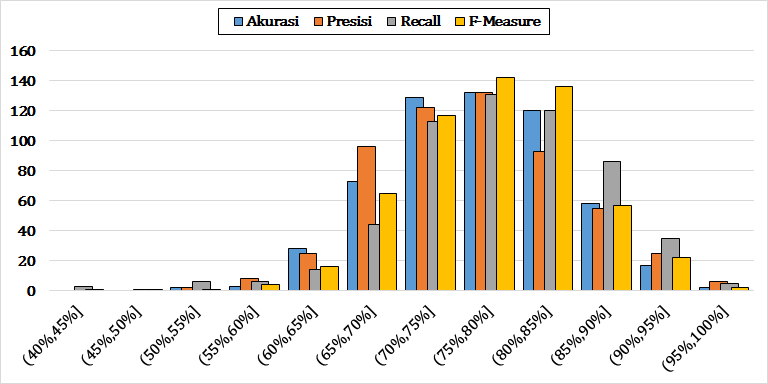
\includegraphics[width=\linewidth]{pics/histogram10}
    \caption{Histogram Metrik Evaluasi dengan Fitur SDCC dan Metode Klasifikasi SVM}
    \label{fig:histogram10}
  \end{figure}

  Dari Gambar \ref{fig:histogram10} dapat diamati bahwa mayoritas ayat dalam eksperimen terklasifikasi dengan rentang akurasi (75\%,80\%]. Hasil tersebut secara signifikan lebih tinggi jika dibandingkan dengan beberapa hasil pada eksperimen yang menggunakan fitur MFCC. Hal tersebut mengindikasikan bahwa penggunaan fitur SDCC lebih tepat daripada fitur MFCC, untuk digunakan dalam sistem evaluasi pembacaan \quran~dalam penelitian ini.





  %-----------------------------------------------------------------------------%
  \subsection{Hasil dengan Fitur SDCC dan Metode Klasifikasi GMM}
  %-----------------------------------------------------------------------------%
  Eksperimen menggunakan fitur SDCC dan menggunakan metode klasifikasi GMM, memberikan hasil yang dirangkum pada Tabel \ref{table:sdccgmm} berikut.

  \begin{table}
    \centering
    \caption{Rangkuman Hasil Eksperimen dengan Fitur SDCC dan Metode Klasifikasi GMM}
    \begin{tabular}{|c|c|c|c|c|}
      \hline
       & Akurasi & Presisi & \f{\f{Recall}} & \f{\f{F-Measure}} \\ \hline
      Minimal         & 67.5\% & 64.6\%  & 55.0\%  & 63.8\% \\ \hline
      Maksimal        & 98.8\% & 100.0\% & 100.0\% & 98.8\% \\ \hline
      Rata-rata       & 83.4\% & 89.0\%  & 76.4\%  & 82.0\% \\ \hline
      Standar Deviasi & 5.61\% & 6.39\% & 8.18\% & 6.33\%  \\ \hline
    \end{tabular}
    \label{table:sdccgmm}
  \end{table}

  Tabel \ref{table:datahistogram11} menunjukkan frekuensi kemunculan persentase tertentu yang dikelompokkan ke dalam interval 5\%.

  \begin{table}
    \centering
    \caption{Frekuensi Kemunculan Interval Persentase pada Eksperimen dengan Fitur SDCC dan Metode Klasifikasi GMM}
    \begin{tabular}{|c|c|c|c|c|}
      \hline
\multicolumn{1}{|c|}{Persentase} & \multicolumn{1}{c|}{\begin{tabular}[c]{@{}c@{}}Frekuensi\\ Nilai Akurasi\end{tabular}} & \multicolumn{1}{c|}{\begin{tabular}[c]{@{}c@{}}Frekuensi\\ Nilai Presisi\end{tabular}} & \multicolumn{1}{c|}{\begin{tabular}[c]{@{}c@{}}Frekuensi\\ Nilai \f{Recall}\end{tabular}} & \multicolumn{1}{c|}{\begin{tabular}[c]{@{}c@{}}Frekuensi\\ Nilai \f{F-Measure}\end{tabular}} \\ \hline
(40\%,45\%{]}  & 0   & 0   & 0   & 0   \\ \hline
(45\%,50\%{]}  & 0   & 0   & 0   & 0   \\ \hline
(50\%,55\%{]}  & 0   & 0   & 3   & 0   \\ \hline
(55\%,60\%{]}  & 0   & 0   & 11  & 0   \\ \hline
(60\%,65\%{]}  & 0   & 1   & 45  & 5   \\ \hline
(65\%,70\%{]}  & 10  & 1   & 94  & 12  \\ \hline
(70\%,75\%{]}  & 36  & 10  & 130 & 56  \\ \hline
(75\%,80\%{]}  & 128 & 41  & 129 & 141 \\ \hline
(80\%,85\%{]}  & 193 & 96  & 83  & 171 \\ \hline
(85\%,90\%{]}  & 138 & 161 & 48  & 119 \\ \hline
(90\%,95\%{]}  & 53  & 155 & 18  & 54  \\ \hline
(95\%,100\%{]} & 6   & 99  & 3   & 6   \\ \hline
    \end{tabular}
    \label{table:datahistogram11}
  \end{table}
  
  Gambar \ref{fig:histogram11} merepresentasikan Tabel \ref{table:datahistogram11} dalam bentuk histogram.
  \begin{figure}
    \centering
    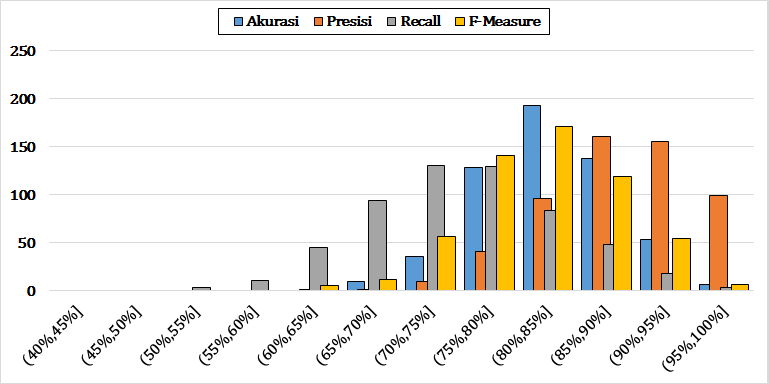
\includegraphics[width=\linewidth]{pics/histogram11}
    \caption{Histogram Metrik Evaluasi dengan Fitur SDCC dan Metode Klasifikasi GMM}
    \label{fig:histogram11}
  \end{figure}

  Dari Gambar \ref{fig:histogram11} dapat diamati bahwa mayoritas ayat dalam eksperimen terklasifikasi dengan rentang akurasi (80\%,85\%]. Hasil tersebut sedikit lebih tinggi jika dibandingkan dengan hasil pada eksperimen yang menggunakan fitur SDCC dan metode klasifikasi SVM. Hal tersebut semakin mengindikasikan bahwa metode klasifikasi GMM lebih tepat untuk digunakan dalam sistem evaluasi pembacaan \quran~dalam eksperimen ini.






  %-----------------------------------------------------------------------------%
  \subsection{Hasil dengan Fitur SDCC dan Metode Klasifikasi Gabungan}
  %-----------------------------------------------------------------------------%
  Eksperimen menggunakan fitur SDCC dan menggunakan metode klasifikasi gabungan SVM dengan GMM, memberikan hasil yang dirangkum pada Tabel \ref{table:sdccgabungan} berikut.

  \begin{table}
    \centering
    \caption{Rangkuman Hasil Eksperimen dengan Fitur SDCC dan Metode Klasifikasi Gabungan}
    \begin{tabular}{|c|c|c|c|c|}
      \hline
       & Akurasi & Presisi & \f{\f{Recall}} & \f{\f{F-Measure}} \\ \hline
      Minimal         & 57.5\% & 56.5\%  & 65.0\%  & 60.5\% \\ \hline
      Maksimal        & 96.3\% & 100.0\% & 100.0\% & 96.4\% \\ \hline
      Rata-rata       & 79.4\% & 77.3\%  & 84.2\%  & 80.4\% \\ \hline
      Standar Deviasi & 6.86\% & 7.80\% & 6.48\% & 6.16\%  \\ \hline
    \end{tabular}
    \label{table:sdccgabungan}
  \end{table}

  Tabel \ref{table:datahistogram12} menunjukkan frekuensi kemunculan persentase tertentu yang dikelompokkan ke dalam interval 5\%.

  \begin{table}
    \centering
    \caption{Frekuensi Kemunculan Interval Persentase pada Eksperimen dengan Fitur SDCC dan Metode Klasifikasi Gabungan}
    \begin{tabular}{|c|c|c|c|c|}
      \hline
\multicolumn{1}{|c|}{Persentase} & \multicolumn{1}{c|}{\begin{tabular}[c]{@{}c@{}}Frekuensi\\ Nilai Akurasi\end{tabular}} & \multicolumn{1}{c|}{\begin{tabular}[c]{@{}c@{}}Frekuensi\\ Nilai Presisi\end{tabular}} & \multicolumn{1}{c|}{\begin{tabular}[c]{@{}c@{}}Frekuensi\\ Nilai \f{Recall}\end{tabular}} & \multicolumn{1}{c|}{\begin{tabular}[c]{@{}c@{}}Frekuensi\\ Nilai \f{F-Measure}\end{tabular}} \\ \hline
(40\%,45\%{]}  & 0   & 0   & 0   & 0   \\ \hline
(45\%,50\%{]}  & 0   & 0   & 0   & 0   \\ \hline
(50\%,55\%{]}  & 0   & 0   & 0   & 0   \\ \hline
(55\%,60\%{]}  & 2   & 6   & 0   & 0   \\ \hline
(60\%,65\%{]}  & 13  & 23  & 3   & 2   \\ \hline
(65\%,70\%{]}  & 49  & 76  & 14  & 26  \\ \hline
(70\%,75\%{]}  & 96  & 123 & 47  & 80  \\ \hline
(75\%,80\%{]}  & 161 & 144 & 119 & 171 \\ \hline
(80\%,85\%{]}  & 137 & 98  & 152 & 154 \\ \hline
(85\%,90\%{]}  & 83  & 60  & 150 & 98  \\ \hline
(90\%,95\%{]}  & 21  & 29  & 71  & 29  \\ \hline
(95\%,100\%{]} & 2   & 5   & 8   & 4   \\ \hline
    \end{tabular}
    \label{table:datahistogram12}
  \end{table}

  Gambar \ref{fig:histogram12} merepresentasikan Tabel \ref{table:datahistogram12} dalam bentuk histogram.
  \begin{figure}
    \centering
    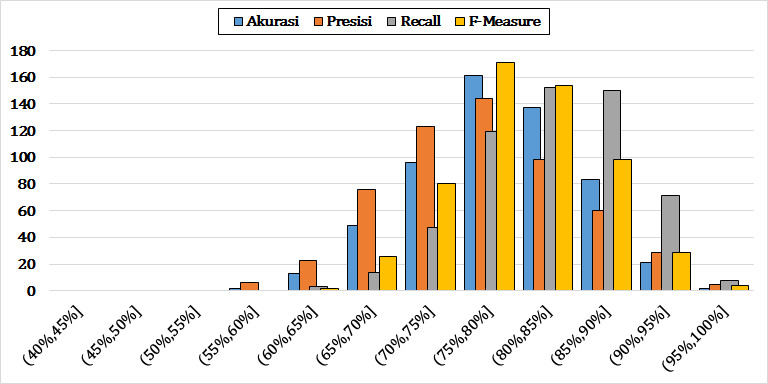
\includegraphics[width=\linewidth]{pics/histogram12}
    \caption{Histogram Metrik Evaluasi dengan Fitur SDCC dan Metode Klasifikasi Gabungan}
    \label{fig:histogram12}
  \end{figure}

  Dari Gambar \ref{fig:histogram12} dapat diamati bahwa mayoritas ayat dalam eksperimen terklasifikasi dengan rentang akurasi (75\%,80\%]. Hasil tersebut sedikit lebih rendah jika dibandingkan dengan hasil pada eksperimen yang menggunakan fitur SDCC dan metode klasifikasi GMM. Hal tersebut semakin mengindikasikan bahwa gabungan dua metode klasifikasi, yaitu SVM dengan GMM, tidak lebih tepat untuk digunakan dalam sistem evaluasi pembacaan \quran~dalam eksperimen ini jika dibandingkan dengan metode klasifikasi GMM.

















%-----------------------------------------------------------------------------%
\section{Perbandingan Hasil}
%-----------------------------------------------------------------------------%

  %-----------------------------------------------------------------------------%
  \subsection{Perbandingan Metode Klasifikasi pada Fitur MFCC}
  %-----------------------------------------------------------------------------%
  Eksperimen menggunakan fitur MFCC dengan berbagai metode klasifikasi, memberikan nilai akurasi yang berbeda-beda pada setiap ayat. Gambar \ref{fig:piefeat0} menunjukkan perbandingan metode klasifikasi yang memiliki nilai akurasi paling tinggi di antara metode-metode yang digunakan dalam eksperimen.

  \begin{figure}
    \centering
    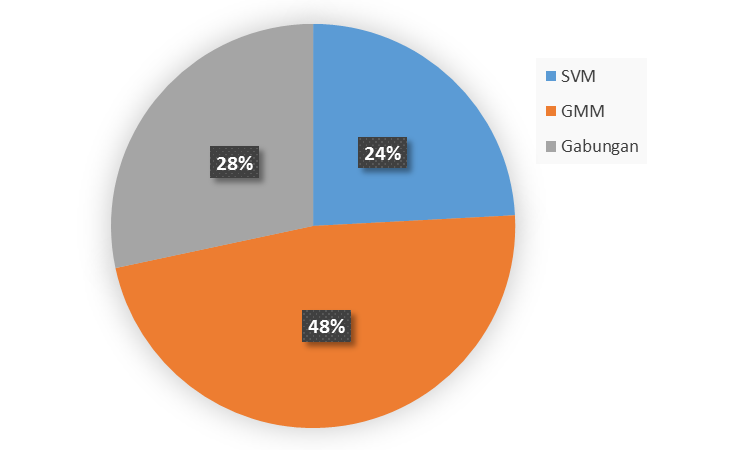
\includegraphics[width=0.9\linewidth]{pics/piefeat0}
    \caption{Perbandingan Metode Klasifikasi untuk Fitur MFCC}
    \label{fig:piefeat0}
  \end{figure}

  Berdasarkan Gambar \ref{fig:piefeat0}, terlihat bahwa pada 48\% ayat dalam eksperimen, metode klasifikasi GMM menghasilkan akurasi tertinggi jika dibandingkan dengan dua metode klasifikasi lainnya. Nilai tersebut mendominasi perolehan akurasi tertinggi pada ketiga metode klasifikasi. Sehingga dapat dikatakan bahwa metode klasifikasi GMM memiliki peluang paling besar untuk menjadi metode yang menghasilkan akurasi tertinggi.



  %-----------------------------------------------------------------------------%
  \subsection{Perbandingan Metode Klasifikasi pada Fitur SDCC}
  %-----------------------------------------------------------------------------%
  Eksperimen menggunakan fitur SDCC dengan berbagai metode klasifikasi, memberikan nilai akurasi yang berbeda-beda pada setiap ayat. Gambar \ref{fig:piefeat1} menunjukkan perbandingan metode klasifikasi yang memiliki nilai akurasi paling tinggi di antara metode-metode yang digunakan dalam eksperimen.

  \begin{figure}
    \centering
    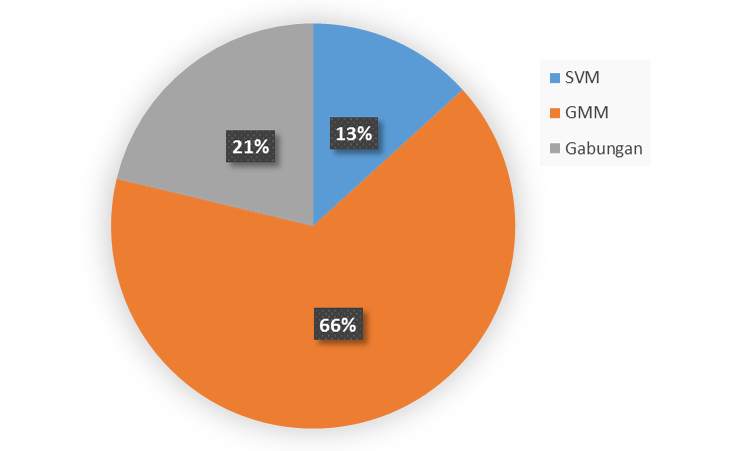
\includegraphics[width=0.9\linewidth]{pics/piefeat1}
    \caption{Perbandingan Metode Klasifikasi untuk Fitur SDCC}
    \label{fig:piefeat1}
  \end{figure}

  Berdasarkan Gambar \ref{fig:piefeat1}, terlihat bahwa pada 66\% ayat dalam eksperimen, metode klasifikasi GMM menghasilkan akurasi tertinggi jika dibandingkan dengan dua metode klasifikasi lainnya. Nilai tersebut mendominasi perolehan akurasi tertinggi pada ketiga metode klasifikasi. Sehingga dapat dikatakan bahwa metode klasifikasi GMM memiliki peluang paling besar untuk menjadi metode yang menghasilkan akurasi tertinggi. Hal tersebut juga konsisten pada eksperimen yang menggunakan fitur MFCC.

  Suatu pembacaan ayat \quran~dapat dinilai benar, salah, jauh dari benar, hampir benar, dan lain sebagainya. Nilai kebenaran suatu pembacaan \quran~tidak bersifat diskrit. Dalam penelitian ini metode klasifikasi GMM lebih banyak menghasilkan akurasi yang lebih tinggi daripada metode klasifikasi SVM karena klasifikasi pembacaan ayat \quran~merupakan klasifikasi yang tidak diskrit, sehingga GMM yang bersifat generatif dapat memodelkan data dengan lebih baik daripada SVM yang bersifat diskriminatif.










  %-----------------------------------------------------------------------------%
  \subsection{Perbandingan Fitur pada Metode Klasifikasi SVM}
  %-----------------------------------------------------------------------------%
  Eksperimen menggunakan metode klasifikasi SVM dengan berbagai fitur, memberikan nilai akurasi yang berbeda-beda pada setiap ayat. Gambar \ref{fig:pieclass0} menunjukkan perbandingan fitur yang memiliki nilai akurasi paling tinggi di antara fitur-fitur yang digunakan dalam eksperimen.

  \begin{figure}
    \centering
    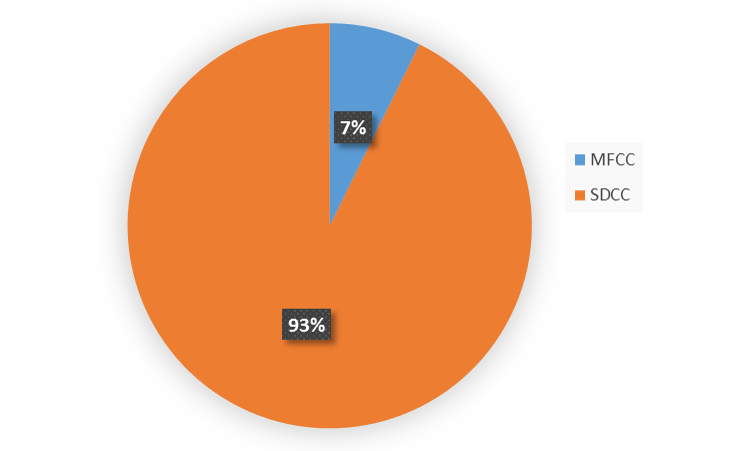
\includegraphics[width=0.9\linewidth]{pics/pieclass0}
    \caption{Perbandingan Fitur untuk Metode Klasifikasi SVM}
    \label{fig:pieclass0}
  \end{figure}

  Berdasarkan Gambar \ref{fig:pieclass0}, terlihat bahwa pada 93\% ayat dalam eksperimen, fitur SDCC menghasilkan akurasi yang lebih tinggi jika dibandingkan dengan fitur MFCC. Nilai tersebut mendominasi perolehan akurasi tertinggi pada kedua fitur. Sehingga dapat dikatakan bahwa fitur SDCC memiliki peluang paling besar untuk menjadi fitur yang menghasilkan akurasi tertinggi.








  %-----------------------------------------------------------------------------%
  \subsection{Perbandingan Fitur pada Metode Klasifikasi GMM}
  %-----------------------------------------------------------------------------%
  Eksperimen menggunakan metode klasifikasi GMM dengan berbagai fitur, memberikan nilai akurasi yang berbeda-beda pada setiap ayat. Gambar \ref{fig:pieclass1} menunjukkan perbandingan fitur yang memiliki nilai akurasi paling tinggi di antara fitur-fitur yang digunakan dalam eksperimen.

  \begin{figure}
    \centering
    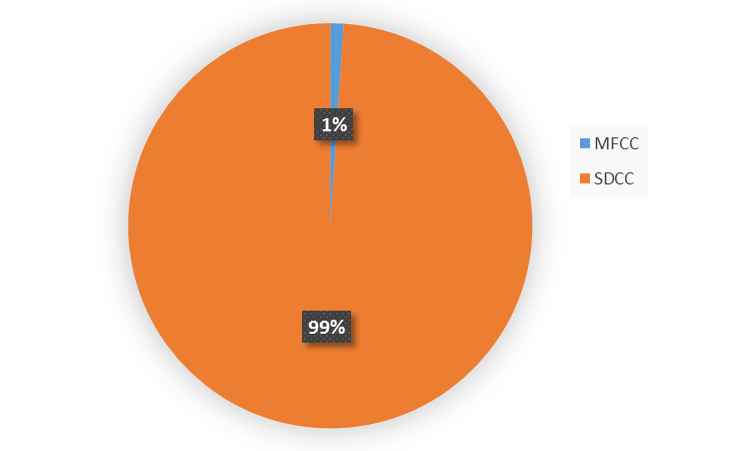
\includegraphics[width=0.9\linewidth]{pics/pieclass1}
    \caption{Perbandingan Fitur untuk Metode Klasifikasi GMM}
    \label{fig:pieclass1}
  \end{figure}

  Berdasarkan Gambar \ref{fig:pieclass1}, terlihat bahwa pada 99\% ayat dalam eksperimen, fitur SDCC menghasilkan akurasi yang lebih tinggi jika dibandingkan dengan fitur MFCC. Nilai tersebut mendominasi perolehan akurasi tertinggi pada kedua fitur. Hal tersebut memperkuat pernyataan bahwa fitur SDCC memiliki peluang paling besar untuk menjadi fitur yang menghasilkan akurasi tertinggi dibandingkan fitur MFCC.




  
  %-----------------------------------------------------------------------------%
  \subsection{Perbandingan Fitur pada Metode Klasifikasi Gabungan}
  %-----------------------------------------------------------------------------%
  Eksperimen menggunakan metode klasifikasi Gabungan dengan berbagai fitur, memberikan nilai akurasi yang berbeda-beda pada setiap ayat. Gambar \ref{fig:pieclass2} menunjukkan perbandingan fitur yang memiliki nilai akurasi paling tinggi di antara fitur-fitur yang digunakan dalam eksperimen.

  \begin{figure}
    \centering
    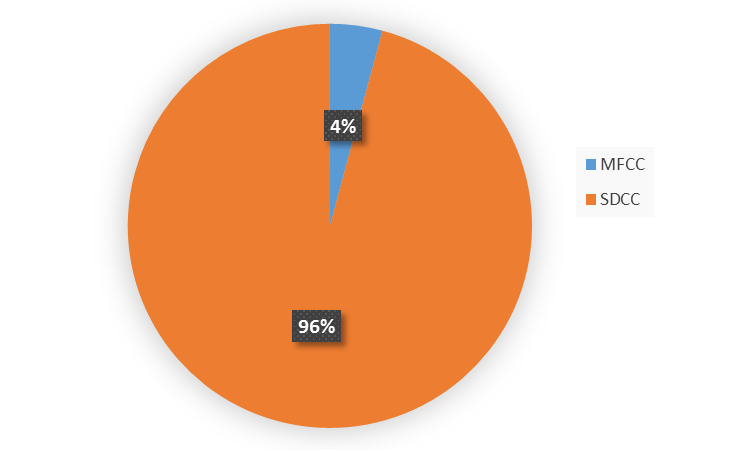
\includegraphics[width=0.9\linewidth]{pics/pieclass2}
    \caption{Perbandingan Fitur untuk Metode Klasifikasi Gabungan}
    \label{fig:pieclass2}
  \end{figure}

  Berdasarkan Gambar \ref{fig:pieclass2}, terlihat bahwa pada 96\% ayat dalam eksperimen, fitur SDCC menghasilkan akurasi yang lebih tinggi jika dibandingkan dengan fitur MFCC. Nilai tersebut mendominasi perolehan akurasi tertinggi pada kedua fitur. Hal tersebut konsisten dengan hasil pada metode klasifikasi SVM maupun GMM, dan semakin memperkuat pernyataan bahwa fitur SDCC memiliki peluang paling besar untuk menjadi fitur yang menghasilkan akurasi tertinggi dibandingkan fitur MFCC.

  Nilai SDCC pada setiap \f{frame} merupakan kombinasi dari beberapa nilai MFCC yang berdekatan. Dalam penelitian ini penggunaan fitur SDCC lebih banyak akurat daripada penggunaan fitur MFCC karena SDCC memuat lebih banyak konteks dalam setiap \f{frame}-nya jika dibandingkan dengan MFCC.











\section{Analisis Lanjut}

Penggunaan fitur SDCC dan metode klasifikasi GMM pada eksperimen memberikan hasil terbaik secara rata-rata, baik pada nilai akurasi, presisi, \f{recall}, ataupun \f{f-measure}. Setiap ayat memiliki hasil klasifikasi yang berbeda-beda. Ada ayat-ayat yang diklasifikasikan dengan akurasi tinggi dan ada juga ayat-ayat yang diklasifikasikan dengan akurasi rendah. Beberapa ayat dengan akurasi tertinggi yang lebih dari atau sama dengan 95\% pada penggunaan fitur SDCC dan metode klasifikasi GMM dapat dilihat pada Tabel \ref{table:akurasitinggi}.

\begin{table}
  \centering
  \caption{Ayat-Ayat yang Diurutkan dari Akurasi Tertinggi}
  \label{table:akurasitinggi}
  \begin{tabular}{|r|r|r|r|r|r|}
  \hline
  Surat & Ayat & Akurasi & Presisi & \f{Recall}  & \f{F-Measure} \\ \hline
  89  & 22 & 98.8\% & 97.6\%  & 100.0\% & 98.8\% \\ \hline
  91  & 13 & 97.5\% & 100.0\% & 95.0\%  & 97.4\% \\ \hline
  92  & 19 & 97.5\% & 97.5\%  & 97.5\%  & 97.5\% \\ \hline
  87  & 7  & 96.3\% & 95.1\%  & 97.5\%  & 96.3\% \\ \hline
  93  & 7  & 96.3\% & 97.4\%  & 95.0\%  & 96.2\% \\ \hline
  110 & 3  & 96.3\% & 100.0\% & 92.5\%  & 96.1\% \\ \hline
  78  & 19 & 95.0\% & 95.0\%  & 95.0\%  & 95.0\% \\ \hline
  79  & 31 & 95.0\% & 97.4\%  & 92.5\%  & 94.9\% \\ \hline
  79  & 46 & 95.0\% & 100.0\% & 90.0\%  & 94.7\% \\ \hline
  80  & 2  & 95.0\% & 100.0\% & 90.0\%  & 94.7\% \\ \hline
  80  & 25 & 95.0\% & 95.0\%  & 95.0\%  & 95.0\% \\ \hline
  88  & 21 & 95.0\% & 100.0\% & 90.0\%  & 94.7\% \\ \hline
  90  & 4  & 95.0\% & 100.0\% & 90.0\%  & 94.7\% \\ \hline
  \end{tabular}
\end{table}


Beberapa ayat dengan akurasi terendah yang kurang dari atau sama dengan 70\% pada penggunaan fitur SDCC dan metode klasifikasi GMM dapat dilihat pada Tabel \ref{table:akurasirendah}.
\begin{table}
  \centering
  \caption{Ayat-Ayat yang Diurutkan dari Akurasi Terendah}
  \label{table:akurasirendah}
  \begin{tabular}{|r|r|r|r|r|r|}
  \hline
  Surat & Ayat & Akurasi & Presisi & \f{Recall}  & \f{F-Measure} \\ \hline
  78    & 4    & 67.5\%  & 71.9\%  & 57.5\% & 63.9\%    \\ \hline
  83    & 4    & 67.5\%  & 64.6\%  & 77.5\% & 70.5\%    \\ \hline
  85    & 21   & 67.5\%  & 69.4\%  & 62.5\% & 65.8\%    \\ \hline
  101   & 10   & 67.5\%  & 71.9\%  & 57.5\% & 63.9\%    \\ \hline
  80    & 24   & 68.8\%  & 75.9\%  & 55.0\% & 63.8\%    \\ \hline
  106   & 1    & 68.8\%  & 75.9\%  & 55.0\% & 63.8\%    \\ \hline
  106   & 3    & 68.8\%  & 74.2\%  & 57.5\% & 64.8\%    \\ \hline
  106   & 4    & 68.8\%  & 71.4\%  & 62.5\% & 66.7\%    \\ \hline
  82    & 12   & 70.0\%  & 73.5\%  & 62.5\% & 67.6\%    \\ \hline
  85    & 6    & 70.0\%  & 76.7\%  & 57.5\% & 65.7\%    \\ \hline
  \end{tabular}
\end{table}

Suatu ayat dapat diklasifikasikan dengan akurasi tinggi dikarenakan ayat tersebut memiliki ciri khusus dalam pelafalannya jika dibandingkan dengan ayat-ayat lainnya. Ciri tersebut antara lain adalah bacaan \f{mad wajib} (bacaan panjang 3 huruf), \f{ghunnah} (bacaan dengung), serta irama panjang pendek dalam pembacaan ayat. Contoh beberapa ayat yang dapat diklasifikasikan dengan akurasi tinggi antara lain sebagai berikut.
\begin{itemize}
  \item Surat ke-89 ayat 22, yaitu ``\<وَجَاءَ رَبُّكَ وَالْمَلَكُ صَفًّا صَفًّا>''. Ayat tersebut mengandung \f{mad wajib} pada kata \<وَجَاءَ> serta \f{ghunnah} pada dua kata \<صَفًّا>.

  \item Surat ke-92 ayat 19, yaitu ``\<وَمَا لِأَحَدٍ عِندَهُ مِن نِّعْمَةٍ تُجْزَىٰ>''. Ayat tersebut mengandung \f{ghunnah} pada kata \<مِن نِّعْمَةٍ>.

  \item Surat ke-110 ayat 3, yaitu ``\<فَسَبِّحْ بِحَمْدِ رَبِّكَ وَاسْتَغْفِرْهُ ۚ إِنَّهُ كَانَ تَوَّابًا>''. Ayat tersebut mengandung \f{ghunnah} pada kata \<إِنَّهُ> dan \<تَوَّابًا>.
\end{itemize}


















% \section{Ayat-Ayat dengan Akurasi Tinggi}

% Berikut adalah beberapa tabel yang berisi ayat-ayat dengan nilai akurasi terbaik.

% \begin{enumerate}
%   \item Tabel \ref{table:topmfccsvm} menampilkan beberapa ayat yang diurutkan berdasarkan akurasi tertinggi pada eksperimen dengan fitur MFCC dan metode klasifikasi SVM.
%   \begin{table}
%     \centering
%     \caption{}
%     \label{table:topmfccsvm}
%     \begin{tabular}{|r|r|r|}
%       \hline
%       \textbf{Surat} & \textbf{Ayat} & \textbf{Akurasi} \\ \hline
%       99    & 7    & 87.5\%  \\ \hline
%       89    & 23   & 85.0\%  \\ \hline
%       91    & 14   & 82.5\%  \\ \hline
%       96    & 11   & 82.5\%  \\ \hline
%       79    & 16   & 81.3\%  \\ \hline
%       78    & 40   & 80.0\%  \\ \hline
%       79    & 45   & 80.0\%  \\ \hline
%       83    & 32   & 80.0\%  \\ \hline
%       84    & 10   & 80.0\%  \\ \hline
%       84    & 11   & 78.8\%  \\ \hline
%       99    & 8    & 78.8\%  \\ \hline
%       102   & 8    & 78.8\%  \\ \hline
%     \end{tabular}
%   \end{table}

%   \item Tabel \ref{table:topmfccgmm} menampilkan beberapa ayat yang diurutkan berdasarkan akurasi tertinggi pada eksperimen dengan fitur MFCC dan metode klasifikasi GMM.
%   \begin{table}
%     \centering
%     \caption{}
%     \label{table:topmfccgmm}
%     \begin{tabular}{|r|r|r|}
%       \hline
%       \textbf{Surat} & \textbf{Ayat} & \textbf{Akurasi} \\ \hline
%       89    & 1    & 85.0\%  \\ \hline
%       84    & 17   & 82.5\%  \\ \hline
%       79    & 45   & 81.3\%  \\ \hline
%       88    & 3    & 81.3\%  \\ \hline
%       106   & 2    & 81.3\%  \\ \hline
%       80    & 41   & 80.0\%  \\ \hline
%       83    & 32   & 80.0\%  \\ \hline
%       110   & 3    & 80.0\%  \\ \hline
%       79    & 46   & 78.8\%  \\ \hline
%       89    & 3    & 78.8\%  \\ \hline
%       89    & 18   & 78.8\%  \\ \hline
%       91    & 10   & 78.8\%  \\ \hline
%     \end{tabular}
%   \end{table}

%   \item Tabel \ref{table:topmfccgabungan} menampilkan beberapa ayat yang diurutkan berdasarkan akurasi tertinggi pada eksperimen dengan fitur MFCC dan metode klasifikasi gabungan.
%   \begin{table}
%     \centering
%     \caption{}
%     \label{table:topmfccgabungan}
%     \begin{tabular}{|r|r|r|}
%       \hline
%       \textbf{Surat} & \textbf{Ayat} & \textbf{Akurasi} \\ \hline
%       91 & 14 & 85.0\% \\ \hline
%       99 & 7  & 83.8\% \\ \hline
%       98 & 1  & 82.5\% \\ \hline
%       79 & 10 & 81.3\% \\ \hline
%       89 & 1  & 81.3\% \\ \hline
%       78 & 37 & 80.0\% \\ \hline
%       79 & 25 & 80.0\% \\ \hline
%       89 & 16 & 80.0\% \\ \hline
%       89 & 22 & 80.0\% \\ \hline
%       96 & 11 & 80.0\% \\ \hline
%     \end{tabular}
%   \end{table}

%   \item Tabel \ref{table:topsdccsvm} menampilkan beberapa ayat yang diurutkan berdasarkan akurasi tertinggi pada eksperimen dengan fitur SDCC dan metode klasifikasi SVM.
%   \begin{table}
%     \centering
%     \caption{}
%     \label{table:topsdccsvm}
%     \begin{tabular}{|r|r|r|}
%       \hline
%       \textbf{Surat} & \textbf{Ayat} & \textbf{Akurasi} \\ \hline
%       81  & 11 & 96.3\% \\ \hline
%       110 & 3  & 96.3\% \\ \hline
%       79  & 27 & 95.0\% \\ \hline
%       89  & 22 & 95.0\% \\ \hline
%       91  & 13 & 95.0\% \\ \hline
%       88  & 3  & 93.8\% \\ \hline
%       95  & 4  & 93.8\% \\ \hline
%       108 & 1  & 93.8\% \\ \hline
%       82  & 2  & 92.5\% \\ \hline
%       86  & 6  & 92.5\% \\ \hline
%       86  & 7  & 92.5\% \\ \hline
%       92  & 19 & 92.5\% \\ \hline
%     \end{tabular}
%   \end{table}

%   \item Tabel \ref{table:topsdccgmm} menampilkan beberapa ayat yang diurutkan berdasarkan akurasi tertinggi pada eksperimen dengan fitur SDCC dan metode klasifikasi GMM.
%   \begin{table}
%     \centering
%     \caption{}
%     \label{table:topsdccgmm}
%     \begin{tabular}{|r|r|r|}
%       \hline
%       \textbf{Surat} & \textbf{Ayat} & \textbf{Akurasi} \\ \hline
%       89  & 22 & 98.8\% \\ \hline
%       91  & 13 & 97.5\% \\ \hline
%       92  & 19 & 97.5\% \\ \hline
%       87  & 7  & 96.3\% \\ \hline
%       93  & 7  & 96.3\% \\ \hline
%       110 & 3  & 96.3\% \\ \hline
%       78  & 19 & 95.0\% \\ \hline
%       79  & 31 & 95.0\% \\ \hline
%       79  & 46 & 95.0\% \\ \hline
%       80  & 2  & 95.0\% \\ \hline
%       80  & 25 & 95.0\% \\ \hline
%       88  & 21 & 95.0\% \\ \hline
%       90  & 4  & 95.0\% \\ \hline
%     \end{tabular}
%   \end{table}

%   \item Tabel \ref{table:topsdccgabungan} menampilkan beberapa ayat yang diurutkan berdasarkan akurasi tertinggi pada eksperimen dengan fitur SDCC dan metode klasifikasi gabungan.
%   \begin{table}
%     \centering
%     \caption{}
%     \label{table:topsdccgabungan}
%     \begin{tabular}{|r|r|r|}
%       \hline
%       \textbf{Surat} & \textbf{Ayat} & \textbf{Akurasi} \\ \hline
%       78  & 19 & 96.3\% \\ \hline
%       110 & 3  & 96.3\% \\ \hline
%       78  & 36 & 95.0\% \\ \hline
%       78  & 39 & 95.0\% \\ \hline
%       79  & 31 & 95.0\% \\ \hline
%       93  & 7  & 95.0\% \\ \hline
%       85  & 12 & 93.8\% \\ \hline
%       89  & 18 & 93.8\% \\ \hline
%       89  & 22 & 93.8\% \\ \hline
%       78  & 14 & 92.5\% \\ \hline
%       80  & 25 & 92.5\% \\ \hline
%       87  & 5  & 92.5\% \\ \hline
%     \end{tabular}
%   \end{table}

% \end{enumerate}

% Dari Tabel {}, ..., diperoleh matriks kemunculan ayat pada tabel {} berikut.
% \begin{table}
%   \centering
%   \caption{}
%   \label{table:kemunculanayatpadatabel}
%   \begin{tabular}{|c|c|c|c|c|c|c|}
%     \hline
%     \textbf{Surat} & \textbf{Ayat} & \textbf{Akurasi} \\ \hline
%     78  & 19 & 96.3\% \\ \hline
%     110 & 3  & 96.3\% \\ \hline
%     78  & 36 & 95.0\% \\ \hline
%     78  & 39 & 95.0\% \\ \hline
%     79  & 31 & 95.0\% \\ \hline
%     93  & 7  & 95.0\% \\ \hline
%     85  & 12 & 93.8\% \\ \hline
%     89  & 18 & 93.8\% \\ \hline
%     89  & 22 & 93.8\% \\ \hline
%     78  & 14 & 92.5\% \\ \hline
%     80  & 25 & 92.5\% \\ \hline
%     87  & 5  & 92.5\% \\ \hline
%   \end{tabular}
% \end{table}

% \section{Ayat-Ayat dengan Akurasi Rendah}
